\documentclass[10pt,a4paper]{article}
\usepackage[utf8]{inputenc}
\usepackage{amsmath}
\usepackage{amsfonts}
\usepackage{amssymb}
\usepackage{amsthm}
\usepackage{float}
\usepackage{mathtools}
\usepackage{geometry}[margin=1in]
\usepackage{xspace}
\usepackage{tikz}
\usepackage{mathrsfs}
\usetikzlibrary{shapes, arrows, decorations.pathmorphing}
\usepackage[parfill]{parskip}
\usepackage{subcaption}
\usepackage{stmaryrd}
\usepackage{marvosym}
\usepackage{dsfont}

\newcommand{\st}{\text{ s.t. }}
\newcommand{\contr}{\lightning}
\newcommand{\im}{\mathfrak{i}}
\newcommand{\R}{\mathbb{R}}
\newcommand{\Q}{\mathbb{Q}}
\newcommand{\C}{\mathbb{C}}
\newcommand{\F}{\mathbb{F}}
\newcommand{\K}{\mathbb{K}}
\newcommand{\N}{\mathbb{N}}
\newcommand{\Z}{\mathbb{Z}}
\renewcommand{\H}{\mathds{H}}
\newcommand{\nequiv}{\not\equiv}
\newcommand{\powset}{\mathcal{P}}
\renewcommand{\th}[1][th]{\textsuperscript{#1}\xspace}
\newcommand{\from}{\leftarrow}
\newcommand{\legendre}[2]{\left(\frac{#1}{#2}\right)}
\newcommand{\ow}{\text{otherwise}}
\newcommand{\imp}[2]{\underline{\textit{#1.}$\implies$\textit{#2.}}}
\let\oldexists\exists
\renewcommand{\exists}{\oldexists\;}
\renewcommand{\hat}{\widehat}
\renewcommand{\tilde}{\widetilde}
\newcommand{\one}{\mathds{1}}
\newcommand{\under}{\backslash}
\newcommand{\injection}{\hookrightarrow}
\newcommand{\surjection}{\twoheadrightarrow}
\newcommand{\jacobi}{\legendre}
\newcommand{\floor}[1]{\lfloor #1 \rfloor}
\newcommand{\ceil}[1]{\lceil #1 \rceil}
\newcommand{\cbrt}[1]{\sqrt[3]{#1}}

\DeclareMathOperator{\ex}{ex}
\DeclareMathOperator{\id}{id}
\DeclareMathOperator{\upper}{Upper}
\DeclareMathOperator{\dom}{dom}

\DeclareMathOperator{\charr}{char}
\DeclareMathOperator{\Image}{im}
\DeclareMathOperator{\ord}{ord}
\DeclareMathOperator{\lcm}{lcm}
\let\emph\relax
\DeclareTextFontCommand{\emph}{\bfseries\em}

\newtheorem{theorem}{Theorem}[section]
\newtheorem{lemma}[theorem]{Lemma}
\newtheorem{corollary}[theorem]{Corollary}
\newtheorem{proposition}[theorem]{Proposition}
\newtheorem{conjecture}[theorem]{Conjecture}

\tikzset{sketch/.style={decorate,
 decoration={random steps, amplitude=1pt, segment length=5pt}, 
 line join=round, draw=black!80, very thick, fill=#1
}}

\title{Automata and Formal Languages}
\begin{document}
\maketitle
\section{Register Machines and Computability}
\textbf{\underline{Books:}} PTJ (Chapter 4)

\textsc{Note: Here $\N = \{0,1,2,\ldots\}$}

A \emph{register machine (RM)} consists of:
\begin{enumerate}
\item A sequence of \emph{registers} $R_1, R_2, R_3, \ldots$ where at discrete time steps $t = 0,1,2,\ldots$ have $R_i(t) \in \N$, In fact, we only have finitely many registers, and regard $R_i \equiv 0$ for all $i\geq I$.
\item A finite \emph{program} consisting of a fixed number of \emph{states} $S_0$ (\textsc{Halt}), $S_1$ (\textsc{Start}), $S_2,\ldots, S_n$. Each state comes with a fixed instruction performed when in state $S_i$. When the computer reaches \textsc{Halt}, we get the output from $R_1$. Otherwise, for $1\leq i\leq n$ we have $2$ types of \emph{commands}:
\begin{enumerate}
\item Increment $R_j$, then move to state $S_k$. We write this $S_i:(j,+,k)$.
\item If $R_j \neq 0$ then decrement $R_j$, then move to state $S_k$. Otherwise move to state $S_l$. We write this $S_i:(j,-,k,l)$.
\end{enumerate}
\end{enumerate}

A \emph{sequence of instructions} for a RM is the ordered list of the instructions for the program.\\
An \emph{input} for a RM is, for some $k\geq 1$, a finite $k$-tuple $(n_1,\ldots,n_k)\in\N^k$ which are the initial values of $R_1,\ldots,R_k$. The other registers are set to 0.

A \emph{program diagram} for a RM is a directed graph with vertices being the states of the machine and the labelled arrows denote the instructions: $S_i:(j,+,k) $

\begin{figure}
\begin{subfigure}{.5\textwidth}
\begin{center}
\tikz{
\node (i) at (0,0) [circle, draw] {$S_i$};
\node (k) at (3,0) [circle, draw] {$S_k$};
\draw (i) edge[->] node[above] {$R_j +1$} (k) ;
}
\end{center}
\caption{$S_i:(j,+,k)$}
\end{subfigure}
\begin{subfigure}{.5\textwidth}
\begin{center}
\tikz{
\node (i) at (0,1) [circle, draw] {$S_i$};
\node (k) at (3,1) [circle, draw] {$S_k$};
\node (l) at (3,0) [circle, draw] {$S_l$};
\draw (i) edge[->] node[above, midway] {$R_j -1$} (k);
\draw (i) edge[dashed,->] (l);
}
\end{center}
\caption{$S_i:(j,-,k,l)$}
\end{subfigure}
\end{figure}

We can then use these to describe programs:
\begin{figure}
\begin{subfigure}{.8\textwidth}
\centering
\tikz{
\node (0) at (0,0) [circle, draw] {$S_0$};
\node (1) at (2,0) [circle, draw] {$S_1$};
\draw[->] (1.-60) arc (220:220+285:6mm) node[midway, right] {$R_1 + 1$};
}
\caption{Repeatedly increment $R_1$, never halting}
\end{subfigure}
\begin{subfigure}{.8\textwidth}
\centering
\tikz{
\node (0) at (0,0) [circle, draw] {$S_0$};
\node (1) at (2,0) [circle, draw] {$S_1$};
\node (2) at (4,0) [circle, draw] {$S_2$};
\node (3) at (6,0) [circle, draw] {$S_3$};
\draw (1) edge[bend left,->] node[above] {$R_2-1$} (2);
\draw (2) edge[bend left,->] node[below] {$R_1-1$} (1);
\draw (1) edge[dashed,->] (0);
\draw (2) edge[dashed,->] (3);
\draw[->] (3.-60) arc (220:220+285:6mm) node[right, midway] {$R_1 + 1$};
}
\caption{For input $(n_1,n_2)$ returns $n_1-n_2$ if $n_1\geq n_2$, else never halt}
\end{subfigure}
\begin{subfigure}{.8\textwidth}
\centering
\tikz{
\node (0) at (1,0) [circle, draw] {$S_0$};
\node (1) at (0,1.5) [circle, draw] {$S_1$};
\node (2) at (2,1.5) [circle, draw] {$S_2$};
\node (3) at (4,1.5) [circle, draw] {$S_3$};
\draw[->] (1.120) arc (40:40+285:6mm) node[left, midway] {$R_j - 1$};
\draw[dashed, ->] (1) edge (2);
\draw (2) edge[->, bend left] node[above] {$R_i-1$} (3);
\draw (3) edge[->, bend left] node[below] {$R_j+1$} (2);
\draw (2) edge[->, dashed, bend left] (0);
}
\caption{Transfer $R_i$ to $R_j$, emptying $R_i$}
\end{subfigure}
\end{figure}

For any $k>0$ a program $P$ \emph{halts} on input $(m_1, m_2, \ldots, m_k) \in \N^k$ if it ever reaches state $S_0$, written $P(m_1,\ldots,m_k)\downarrow$\\
The \emph{halting set} $\Omega(P)$ is a set of inputs on which $P$ halts.
\begin{align*}
\Omega(P) = \cup_{k>0} \{(m_1,\ldots,m_k) : P(m_1,\ldots,m_k)\downarrow\}
\end{align*}
If $P$ does not halt, we write $P(m_1,\ldots,m_k)\uparrow$.

For each program $P$, the \emph{upper register index} $\upper(P)$ is the largest index of a register appearing in the instructions for $P$. So if $i>\upper(P)$ then $R_i$ never changes.

A \emph{partial function} $f:\N^k \rightarrow \N$ is one where the domain of $f$ is a subset of $\N^k$, and undefined otherwise. If $f$ is defined everywhere then we call it a \emph{total function}. This lets us define these programs as functions - we say $f$ is \emph{partial computable} by a program $P$ such that $\forall (m_1,\ldots,m_k) \in \dom(f)$ have $P(m_1,\ldots,m_k)\downarrow$ with $f(m_1,\ldots,m_k) = R_1$ on halting, and $\forall (m_1,\ldots,m_k)\notin \dom(f)$ we have $P(m_1,\ldots,m_k)\uparrow$. Hence any program $P$ and $k>0$ gives a partial function $f:\N^k \rightarrow \N$.

\begin{lemma}
We can add $R_i$ to $R_j$ leaving $R_i$ unchanged.
\end{lemma}
\begin{proof}
\item
\centering
\tikz{
\node (1) at (0,4) [circle,draw] {$S_1$};
\node (2) at (2,4) [circle,draw] {$S_2$};
\node (3) at (4,4) [circle,draw] {$S_3$};
\node (4) at (1,2) [circle,draw] {$S_4$};
\node (5) at (3,2) [circle,draw] {$S_5$};
\node (0) at (0,0) [circle,draw] {$S_0$};
\draw (1) edge[->] node[below] {$R_i-1$} (2);
\draw (2) edge[->] node[below] {$R_n+1$} (3);
\draw (1) edge[->, dashed] (4);
\draw (3) edge[->, bend right] node[above] {$R_j+1$} (1);
\draw (4) edge[->, bend left] node[above] {$R_n-1$} (5);
\draw (5) edge[->, bend left] node[below] {$R_i+1$} (4);
\draw (4) edge[->, dashed] (0);
}\\
Thus by setting ($i=2, j=1$) we see that $(n_1, n_2) \mapsto n_1 + n_2$ is total computable.
\end{proof}
We have already seen that the function $n\mapsto 0$ is also computable. This can be done with the machine:
\begin{center}
\tikz{
\node (1) at (0,0) [circle, draw] {$S_1$};
\node (0) at (2,0) [circle, draw] {$S_0$};
\draw (1) edge[->, dashed] (0);
\draw[->] (1.120) arc (40:40+285:6mm) node[left, midway] {$R_1 - 1$};
}
\end{center}
\begin{corollary}
There exists a routine which can copy $R_i$ to $R_j$ leaving $R_i$ unchanged.
\end{corollary}
\begin{proof}
First empty $R_j$, then use \textbf{1.1} to add $R_i$ to $R_j$.
\end{proof}
We can use these as subroutines to join with other programs $P$. Use registers $R_n \st n> \upper(P)$ and largest input register. Then replace the halt state of $P$ with the start state of the subroutine. In fact we have already done this - if you look carefully at the adding machine, you can see that the middle section is the same as the machine in (c) of the examples - this is the part where we replace the value in $R_i$ from its temporary location in $R_n$.

\subsection*{Partial Recursive Functions}
Partial computable functions have good closure properties.
\begin{theorem}
\item
\begin{enumerate}
\item For $i\leq k$, the \emph{projection function} $(n_1, \ldots, n_k) \mapsto n_i$ is computable.
\item The zero function $n\mapsto 0$ and \emph{successor function} $n\mapsto n+1$ are computable
\item (Composition) If $f:\N^k\rightarrow \N$ and $g_1, \ldots, g_k:\N^{l} \rightarrow \N$ are all partial computable then so is the composition function $h(n_1,\ldots,n_l) = f(g_1(n_1,\ldots,n_l),\ldots,g_k(n_1,\ldots,n_l))$ where defined. If $f,g_1,\ldots,g_k$ are total functions, so is $h$.
\item (Recursion) If $f$ on $k$ variables and $g$ on $k+2$ variables are partial computable, then so is the partial function $h:\N^{k+1}\rightarrow \N$ defined inductively as:
\begin{align*}
h(n_1,\ldots,n_k,0)&=f(n_1,\ldots,n_k)\\
h(n_1,\ldots,n_k,n_{k+1}+1) &= g(n_1,\ldots,n_{k+1},h(n_1,\ldots,n_{k+1}))
\end{align*}
Moreover, $f,g$ total $\implies h$ total.
\item (Minimisation) If $f$ on $k+1$ variables is partial computable then so is the partial function $g:\N^k\rightarrow \N$ defined by $g(n_1,\ldots,n_k) = n$ if $f(n_1,\ldots,n_k,n) = 0$ and $f(n_1,\ldots,n_k,m) > 0$ for all $m<n$, and is undefined if no zero is ever found. Note that $f$ total $\nRightarrow g$ total.
\end{enumerate}
\end{theorem}
\begin{proof}\item
\begin{enumerate}
\item We can use the program Transfer $R_i$ to $R_1$, \textsc{Halt}.
\item Zero function has already been seen. For successor function, use:
\begin{center}
\tikz{
\node (1) at (0,0) [circle, draw] {$S_1$};
\node (0) at (2,0) [circle, draw] {$S_2$};
\draw (1) edge[->] node[above] {$R_1 +1$} (0);
}
\end{center}
\item First transfer $R_1,\ldots, R_l$ to $R_{N+1},\ldots, R_{N+l}$ where $N$ is large enough to not be needed in other subroutines. Then for each $1\leq i\leq k$ in turn, copy $R_{N+1}, \ldots, R_{N+l}$ to $R_{k+1},\ldots, R_{k+l}$, perform $g_i$ but with all registers shifted up by $k$ and then transfer answer from $R_{k+1}$ to $R_{i}$, then clear $R_{k+2},\ldots,R_N$. Finally, apply $f$. 
\item Copy $R_1,\ldots,R_k$ to $R_{N+1},\ldots,R_{N+k}$, transfer $R_{k+1}$ to $R_{N+k+2}$ (``counts down"), then do $f$. Then:
\begin{center}
\tikz{
\node (0) at (0,3) [circle, draw] {$\cdot$};
\node[draw] (1) at (7,2) {Transfer $R_1$ to $R_{k+2}$ then copy $R_{N+1},\ldots, R_{N+k+1}$ to $R_1,\ldots,R_{k+1}$};
\node (2) at (5,0) [draw] {\textsc{Halt}$(g)$, clear $R_{k+2},\ldots,R_N$};
\node (3) at (0,0) [draw] {\textsc{Halt}};
\draw (0) edge[->, bend left] node[above] {$R_{N+k+2} -1$} (1);
\draw (1) edge[->] node[right] {$g$} (2);
\draw (2) edge[->, bend left] node[right] {$R_{N+k+1}+1$} (0);
\draw (0) edge[->, dashed] (3);
}
\end{center}
\item Copy $R_1, \ldots, R_k$ to $R_{N+1},\ldots,R_{N+k}$. Then
\begin{center}
\tikz{
\node (0) at (1,2) [circle, draw] {$\cdot$};
\node[draw] (1) at (2,4) {Copy $R_{N+1},\ldots,R_{N+k+1}$ to $R_1,\ldots,R_{k+1}. $ Clear $R_{k+2},\ldots, R_N$};
\node (2) at (2,0) [draw] {\textsc{Halt}$(f)$};
\node (3) at (6,0) [draw] {Transfer $R_{N+k+1}$ to $R_1$, \textsc{Halt}};
\draw (0) edge[->] node[left] {$R_{N+k+1} +1$} (1);
\draw (1) edge[->] node[right] {$f$} (2);
\draw (2) edge[->] node[left] {$R_{i}-1$} (0);
\draw (2) edge[->, dashed] (3);
}
\end{center}
\end{enumerate}
\end{proof}
The class of \emph{partial recursive functions} is the smallest class of partial functions from $\N^k$ to $\N$ over all $k\geq 1$ closed under the operations \textbf{1.3} (1) to (5). That is, $f$ can be constructed from basic functions and applications of $(3), (4), (5)$ a finite number of times.

So \textbf{1.3} says that partial recursive $\implies$ partial computable.

A partial function is \emph{primitive recursive} if we never use \textbf{1.3} (5) its construction. Note that primitive recursive $\implies$ total recursive, as (5) was the only construction that breaks the totality of the function. [The converse implication is not true: the Ackermann function.]

Example: $+$ and $\times$ are primitive recursive:
\begin{itemize}
\item[$+$:] Let $h(m,0) = m$, $h(m,n+1) = h(m,n) + 1 = g(m,n,h(m,n))$, where $g(x,y,z) = z+1$.
\item[$\times$:] $H(m,0) = 0$, $H(m,n+1) = H(m,n) + m = g(m,n,H(m,n))$ for $g(x,y,z) = x+z$.
\end{itemize}
Example: $(m,n)\mapsto m^n$ is primitive recursive - left as exercise.

We need to be able to ``encode" finite sequences of arbitrary length in $\N$. For $n>0$ and $i\in\N$, write $p_i$ for the $(i+1)\th$ prime (so $p_0 = 2$). Write $(n)_i$ for the largest power of the prime $p_i$ that divides $n$.

\begin{lemma}
For each fixed $i$, the 1 variable function $(\cdot)_i : \N \rightarrow \N$ is primitive recursive.
\end{lemma}

\begin{proof}
First note that, for any finite sequence $(m_0, m_1, \ldots, m_s)\subseteq\N^{s+1}$, the function\\ $f(n) = \begin{cases} m_n &n\leq s \\ 0 & n>s \end{cases}$ is primitive recursive.

By induction on $s$ and recursion from \textbf{1.3} \textit{(4)}, for $k=0$ if $c$ constant and $g:\N^2 \rightarrow \N$ is primitive recursive, then so is $h(0) = c, h(n+1) = g(n, h(n))$.

Thus, given $f:\N\rightarrow\N$ primitive recursive, let $g(n,m) \coloneqq f(n)$, which is primitive recursive. So $h(0)=c, h(n+1)=f(n)$ is primitive recursive, and we can repeat this process. 

This includes for each \underline{fixed} k:
\begin{enumerate}
\item The step function $\text{Step}_k(n) = \begin{cases} 1 & 0\leq n\leq k-1 \\ 0 & \text{otherwise} \end{cases}$
\item The delta function $\delta_k(n) = \begin{cases} 1 & n=k \\ 0 & n\neq k\end{cases}$ Let $\epsilon(n) = \delta_0(\delta_0(n)) = \begin{cases} 0 & n=0\\ 1 & n=1\end{cases}$ - this is also primitive recursive.
\item The slope function $\text{Slope}_k(n) = \begin{cases} n+1 & 0\leq n \leq k-2 \\ 0 & \text{otherwise} \end{cases}$
\item The remainder function $\text{Rem}_k(n) = n \mod k$ use recursion in the form $g(n,m) \coloneqq f(m)$, so $h(0) = 0$, $h(n+1)=f(h(n))$ primitive recursive if $f$ is. Here, $\text{Rem}_k(n+1) = \text{Slope}_k(\text{Rem}_k(n))$
\item[*5.] $\text{Floor}_k(n) = \left\lfloor\frac{n}{k}\right\rfloor$
\item[*6.] $\text{Divide}_k(n) = \begin{cases} n/k & n\equiv 0 \mod k \\ 0 & \text{otherwise} \end{cases}$
\item[*7.] Division by powers $\text{Power}_k(n,m) = \begin{cases} n/k^m & n\equiv 0 \mod k^m \\ 0 & \text{otherwise} \end{cases}$
\item[*8.] $\text{Maxpower}_k(n) = \begin{cases} 0 & n=0 \\ \text{largest power of k dividing n} & n\neq 0 \end{cases}$
\end{enumerate}
Proofs of *ed function are on example sheet 1.

Now define by recursion $h(n,0) = 0$ and $h(n,m+1) = h(n,m) + \epsilon(\text{Power}_k(n,m+1))$.\\
$\epsilon(\text{Power}_k(n,j)) = \begin{cases} 1 & k^j \text{ divides } n>0 \\ 0 & \text{otherwise} \end{cases}$, so is $0$ if $j\geq n$

So $h(n,n) = \sum_{i=1}^n \epsilon(\text{Power}_k(n,1)) = \text{Maxpower}_k(n)$, so $h(n,n)$ is primitive recursive.
\end{proof}

\subsection*{Computable = Recursive}
We have seen already that partial recursive $\implies$ partial computable.
\begin{theorem}
Every partial computable function $f:\N^k \rightarrow \N$ is partial recursive.
\end{theorem}
\begin{proof}
From a program $P$ for $f$, define $g:\N^{k+2}\rightarrow \N$, ``what actually goes on in $P$", to be the function:
\begin{center}
$g(n_1,\ldots,n_k,0,t) $ is the state of $P$ after time $t$ with input $(n_1,\ldots,n_k)$
\end{center}
So $t=0$ gives $1$ and if halt at $t_0$ then gives $0$ for all $t \geq t_0$, and:
\begin{center}
$(n_1, \ldots, n_k, i, t)$ is the contents of $R_i$ at time $t$
\end{center}
So have $N$ (assume $>k$) such that $g(\cdots, i, \cdot) = 0 \forall i>N$. Note that $g$ is a total function.

\underline{Suppose} that $g$ is recursive and define $q(n_1,\ldots, n_k) = \min\{t: g(n_1,\ldots,n_k,0,t)=0\}$. Then $q$ is partial recursive, and so $f(n_1, \ldots, n_k) = g(n_1, \ldots, n_k, 1, q(n_1, \ldots, n_k))$ is partial recursive.

\underline{Proof that $g$ is recursive:}\\
Fix $n_1, \ldots, n_k$ and $t$. For each $0\leq i \leq N$, $g$ gives $(g_0, \ldots, g_N) \in \N^{N+1}$, encode as $c(d_0, \ldots, d_N) = 2^{d_0}3^{d_1}\ldots p_N^{d_N} \in \N$ is primitive recursive. Also, $(c(d_0, \ldots, d_N))_i = d_i$ is primitive recursive. We will define $h:\N^{k+2}\rightarrow \N$ via recursion where $h(n_0, n_1, \ldots, n_k, t)$ is the coded integer of state and registers of $P$ at time $t$ for input $n_1, \ldots, n_k$ and start state $n_0$ (here $=1$).

In particular, for $t=0, h=2^{n_0}3^{n_1}\ldots p_k^{n_k}$. For recursion for $h$, we need $s:\N\rightarrow\N$, the ``transition function", which computes in coded form the changes at each step.
\end{proof}

\subsection*{Algorithms and Recursive Sets}
A function $f:\N^k \rightarrow \N$ is \emph{recursive} or \emph{computable} if it is total. If it s not even partial recursive, then it is \emph{incomputable}.

A subset $X\subseteq \N^k$, (often $X\subseteq \N$) is \emph{recursive} or \emph{computable} or \emph{decidable} if the characteristic function $\chi_X(n) = \begin{cases} 1 & n\in X \\ 0 & n \notin X\end{cases}$ is computable, i.e. if we can program a computer to tell us if a given number is in it or not.

An \emph{algorithm} is any process which takes an input in $\N^k$ for some specified $k$, or a recursive subset $X\subseteq \N^k$, and returns an output in $\N$ which is simulated by a register machine.

A \emph{total algorithm} terminates for all elements in $X$, whilst a \emph{partial algorithm} may fail to terminate for some choices of input.

\begin{lemma}
For each $k\geq 1$, there is some total function $f:\N^k \to \N$ which is incomputable.
\end{lemma}
\begin{proof}
Each computable program comes from a finite program with $n+1$ states for some $n$. Since there are only countably many finite programs, but $\powset(\N)$ is uncountable, hence one of these sets is not computable. Then its indicator function is not computable.
\end{proof}

For given $m$, the \emph{shortlex} ordering on $\N^m$ is $(n_1,\ldots, n_m) < (n_1', \ldots, n_m')$ if $\sum n_i < \sum n_i'$ or $\sum n_i = \sum n_i$ and there is some $j$ with $n_i = n_i'$ for $i<j$, but $n_{j+1} > n'_{j+1}$.

This gives us a bijection to $\N$, as there are only finitely many $k$-tuples of naturals with sum less than $N \in \N$.

If a register machine $P$, then for the $i$\th instruction, let $t_i = \begin{cases} 2^j \cdot 5^k & \text{if it is } (j, +, k) \\ 2^j\cdot 3\cdot 5^k \cdot 7^l & \text{if it is } (j,-,k,l)\end{cases}$. We can then encode the tuple $(t_1, t_2, \ldots, t_n)$ as $m=2^n\cdot 3^{t_1}\cdot 5^{t_2} \cdot\ldots \cdot p_n^{t_{n-1}}$. We denote the program encoded by the number $m$ as $P_m$, if $m$ is a valid encoding of a program. For these $m$, we say $m$ \emph{codes} a program, and $P_m$ is the \emph{m\th machine}.

The input for a register machine is a $k$-tuple for varying $k$, so we define $f_{n,k}$ for the $k$-variable function computed by the $n$\th machine if $P_n$ exists.

Here is an explicit total function which is not recursive:
\begin{lemma}
Consider the following function $g:\N\to\N$ given by:
\begin{align*}
g(n) \coloneqq \begin{cases} f_{n,1}(n) + 1 & \text{if $n$ codes a program and if $f_{n,1}(n)$ is defined} \\ 0 & \text{else}\end{cases}
\end{align*}
Then $g$ is not recursive.
\end{lemma}
\begin{proof}
If $g$ is recursive then it is computed by some machine. So there exists an $N$ such that $g = f_{N,1}$ is total. But then $f_{N,1}(N) = g(N) = f_{N,1}(N) + 1$ \contr.
\end{proof}

\subsection*{Church's Thesis}
The two key figures in this chapter are Alonzo Church and Alan Turing, doing this work around 1936.

An \emph{executable process} is a step-by-step deterministic process with finite description at each step, a finite set of rules, and a finite amount of input and output.

An \emph{abstract theory of finite computation} is a theory of computation consisting of these executable processes.

\begin{theorem}[Church's Thesis]\item
\begin{enumerate}
\item In any abstract theory of finite computation, $\mathscr{C}$, the $\mathscr{C}$-partial computable function $f:\N^k \to \N$ gives at most the partial recursive functions.
\item Any informal description of an executable process starting with input in $\N^k$ and output in $\N$ or never halting is equivalent to a register machine, so we don't need to worry about all the details of the machine.
\item There is a total algorithm, that, given the encoding (e.g. shortlex) of a description of an algorithm, returns a code for a register machine that carries out this process.
\end{enumerate}
\end{theorem}
This is not so much one theorem as many different independent theorems. It has however been proven that all the following abstract theories of finite computation are equivalent:
\begin{itemize}
\item Church's $\lambda$-calculus
\item Turing machines
\item Register machines
\item Standard languages
\item Quantum/DNA-computers
\end{itemize}
From now on, we will refer to these three statements as ``Church's thesis" or even just ``Church". 

\begin{lemma}
Let $h:\N\rightarrow \N$ be:
\begin{align*}
h(n) = \begin{cases}f_{n,1} (n) + 1 & \text{if $n$ codes a program and $f_{n,1}(n)$ defined} \\ \text{undefined} & \text{otherwise}\end{cases}
\end{align*}
Then $h$ is partial recursive.
\end{lemma}

\begin{proof}
For input $n$, check if $n$ codes a program - this is total recursive. If so, run the program with input $n$. If it then halts, add $1$ to $R_1$ and halt, and so by Church $h$ is partial computable = partial recursive.
\end{proof}

\subsection*{Recursively Enumerable Sets}
Given a partial recursive function $f:\N^k \to \N$ with domain $X\subseteq \N^k$, suppose we input $7$. If $f(7)\downarrow$, then we can run the machine and get the answer within finite time. However, if $f(7)\uparrow$, then we will be waiting forever. By the halting problem, there is no way to know in advance what will happen.

Now suppose we ask: ``Does $f$ halt on either $7$ or $9$?" Then the answer is yes, but if we are unlucky and start with $9$, we will never know if we na\"ively compute $f(9)$, then $f(7)$. 

So instead, we zig-zag: we do one step of each alternately.\\
Let $P_n^t(x)$ be the $t\th$ step of $P_n$ with input $x$. Then we can do:
\begin{center}
\tikz{
\node (1) at (0,3) {$P_n^1(7)$};
\node (2) at (4,3) {$P_n^1(9)$};
\node (3) at (0,2) {$P_n^2(7)$};
\node (4) at (4,2) {$P_n^2(9)$};
\node (5) at (0,1) {$P_n^3(7)$};
\node (6) at (4,1) {$P_n^3(9)$};
\node (7) at (0.5,0.2) {};
\draw[->] (1) edge (2) (2) edge (3) (3) edge (4) (4) edge (5) (5) edge (6);
\draw[dotted, ->] (6) edge (7);
}
\end{center}
We can clearly extend this to any set of finite size. We can even do infinite sets, by following a path similar to in the textbook enumeration of $\Q$:
\begin{center}
\tikz{
\node (1) at (0,3) {$P_n^1(1)$};
\node (2) at (2,3) {$P_n^1(2)$};
\node (3) at (0,2) {$P_n^2(1)$};
\node (4) at (0,1) {$P_n^3(1)$};
\node (5) at (2,2) {$P_n^2(2)$};
\node (6) at (4,3) {$P_n^1(3)$};
\node (7) at (4,2) {$P_n^2(3)$};
\node (8) at (2.5,1.2) {};
\draw[->] (1) edge (2) (2) edge (3) (3) edge (4) (4) edge (5) (5) edge (6) (6) edge (7);
\draw[dotted, ->] (7) edge (8);
}
\end{center}
We can even alternate between different machines, and this process can be extended to any countable set. Then by Church, we can write a program that returns $1$ for input $x \in \N^k, k < \infty$ if some partial recursive function $f$ halts on input of $x$.

We say a set $E\subseteq \N^k$ is \emph{recursively enumerable} if the function
\begin{align*}
\phi_E(n) \coloneqq \begin{cases} 1 & n\in E \\ \uparrow&  \text{else}\end{cases}
\end{align*}

The idea behind this definition is that, compared to a recursive set, here we can only say that $x$ is in $E$, whereas in a recursive set we can say if $x \in E$ or $x \notin E$. A consequence of this is that, by applying the above process for $\phi_E$ on all of $\N^k$, we will eventually get out all the elements of $E$, but we will not know when this has happened (indeed, it might take infinitely long to get all the elements, but we will eventually be notified that any given element is in $E$), so we can ``recursively enumerate" $E$. Conversely, recursive sets are often called \emph{decidable} - we can always decide whether or not $x \in E$. We will cement this discussion into a few theorems now:

\begin{theorem}
The following are equivalent for any subset $E \subseteq \N$:
\begin{enumerate}
\item $E$ is the range of some partial recursive function on some number of variables, i.e.\\ $E = \{f_{n,k}(\mathbf{x}) : \mathbf{x} \in \N^k\}$
\item $E$ is the domain of definition of some partial recursive function on $1$ variable, i.e.:
$\exists n \st E = \{m\in\N : f_{n,1}(m)\downarrow\}$
\item $E$ is recursively enumerable
\item The function $\psi_E(n) = \begin{cases} n & n \in E \\ \uparrow & \ow \end{cases}$ is partial recursive. i.e. we can enumerate the elements of $E$ in a recursive fashion.
\end{enumerate}
\end{theorem}
\begin{proof}\item
\begin{itemize}
\item{\imp{2}{3}} Given a program $P_n$ for computing $f_{n,1}$, modifying at end so it empties $R_1$ then adds $1$.
\item{\imp{3}{4}} Similarly, we start by copying $R_1$ to $R_N$ for large enough $N$, then at the end empty $R_1$ and copy $R_N$ to $R_1$.
\item{\imp{4}{1}} Immediate as $f_{n,k} = \psi_E$ for some choice of $n$, $k=1$.
\item{\imp{1}{2}} Given a program $P_n$ for computing $f_{n,k}:\N^k \to \N$ with range $E$, do the following process $Q$ by Church:

Given an input $x\in \N$ for $Q$, run a zig-zag procedure having ordered $\N^k$ to compute $f_{n,k}(\cdot)$ for each input $\cdot \in \N^k$. Each time, $f_{n,k}(m_1,\ldots, m_k)$ halts, run the total subroutine comparing the output to $x$ wand halt with output $1$ if equal. If not, return to the zig-zag process. So $Q$ will return $1$ if $x$ is in the range $f_{n,k}$, and if not will run forever, because we would never get an output equalling $x$.
\end{itemize}
\end{proof}

\subsection*{Properties of Recursively Enumerable Sets}
In \textbf{1.10}(\textit{1.}), can we have a total recursive function?
\begin{theorem}
If $E \neq \emptyset$ and $E\subseteq \N$, then $E$ is recursively enumerable if and only if $E$ is the range of a total recursive function $f:\N \to \N$.
\end{theorem}
\begin{proof}
For $E = \{e_0, \ldots, e_{k-1}\}$ finite, define $f(n)\coloneqq \begin{cases} e_n & n <k \\ e_{k-1} & \ow\end{cases}$. This is total recursive.

In the case of infinite $E \subseteq \N$ which is the domain of a partial recursive function $g:\N \to \N$, run a zig-zag process to perform the steps of computing $g(0), g(1), \ldots$. Define a total function $f:\N\to\N$ as $f(0)$ is the first input number $i$ for which the computation of $g(i)$ halts in this process (not necessarily the smallest), $f(1)$ the second, and so on. Thus the range of $f$ is $E$ and $f$ is recursive by Church.
\end{proof}

So each program $P_n$ corresponds to a recursively enumerable set which is the domain of $f_{n,1}$. Thus let $W_n = \{x\in\N : f_{n,1}(x) \downarrow \}$ if $n$ encodes a program, and the empty set otherwise. We say $W_n$ is the \emph{n\th recursively enumerable set}, though the labelling is not unique, i.e. it could be that $W_n = W_m$ for some $n\neq m$.

Every recursive subset is recursively enumerable by definition. However:
\begin{theorem}
For any $E\subseteq \N$, $E$ is recursive if and only if $E$ and $\N\setminus E$ is recursively enumerable.
\end{theorem}
\begin{proof}\item
\begin{itemize}
\item{\underline{$\implies$}} As $\chi_E$ is total recursive, $\phi_E$ is partial recursive because when $\chi_E$ halts, if the output is 1 then halt, otherwise enter an infinite loop. We can do the same for $\N\setminus E$, to get $\phi_E, \phi_{\N\setminus E}$.
\item{\underline{$\impliedby$}} As $\phi_E$ and $\phi_{\N\setminus E}$ are both partial recursive, we can do a zig-zag process between the two. Then, if $\phi_E(x)$ halts, return $1$, otherwise if $\phi_{\N\setminus E}(x)$ halts, return $0$. Since $E \cup \N\setminus E = \N$, exactly one of these will halt, and so this gives $\chi_E$ which is total recursive.
\end{itemize}
\end{proof}

\begin{theorem}\item
\begin{enumerate}
\item If $I \subseteq \N$ is recursively enumerable, then the union $\cup_{n\in I} W_n$ is recursively enumerable.
\item If $J \subseteq \N$ is finite, then $\cap_{n\in J} W_n$ is recursively enumerable.
\end{enumerate}
\end{theorem}
\begin{proof}\item
\begin{itemize}
\item[\textit{1.}] We want a process that, given an input $x \in \N$, halts if $x \in \cup_{n\in I}W_n$, and not if $x \notin \cup_I W_n$.

By a big zig-zag process, start outputting elements $n$ of $I$, test if $n$ codes a program $P_n$, move on if not but if so, start to run $P_n$ on this input $x$. One of these subprocesses halts if and only if $x \in W_n$ for some $n \in I$, in which case halt the whole process. However, if $x \notin \cup_I W_n$, then the process will run forever.

\item[\textit{2.}] First check all the $j \in J$ code a program, else we have $\emptyset$. Then run these $|J|$ programs in parallel, each with input $x$. If/when all of these halt, then halt. Then we halt if and only if $x \in \cap_J W_n$.
\end{itemize}
\end{proof}

\subsection*{Universality and Undecidability}
Turing's paper was titled ``On computable numbers, with an application to the Entscheidungsproblem", published in the Proceedings of the London Mathematical Society 42 (1936) pp. 230-265.

\begin{theorem}[Existence of universal programs]
There exists a partial recursive function $u:\N^3 \to \N$ such that:
\begin{align*}
u(n,k,m) = \begin{cases} r & n \text{ codes a program and $m$ codes a $k$-tuple and $f_{n_k}((m)_1,\ldots,(m)_k) = r$} \\
\uparrow & \ow \end{cases}
\end{align*}
\end{theorem}
\begin{proof}
On input, check if $n$ codes a program. If not, loop forever. If so, decode $m$ and see if it is a $k$-tuple, else loop forever. If so, then run the program defined by $n$ on input $((m)_1, \ldots, (m)_k)$. If it halts, output $r$, the contents of $R_1$, otherwise just leave it running.
\end{proof}

There exist subsets of $\N$ which are recursively enumerable but not recursive. We will give a specific example of one: the \emph{halting set} or $\H$.
\begin{align*}
\H \coloneqq \left\{ (n,m) : n \text{ codes a program and } f_{n,1}(m)\downarrow \right\} \subseteq \N^2
\end{align*}
We also define:
\begin{align*}
\K \coloneqq \left\{ n : n \text{ codes a program and } f_{n,1}(n)\downarrow \right\} \subseteq \N
\end{align*}
Observe $\K\times \K \subseteq \H$.
\begin{theorem}[Undecidability of the Halting Problem]
The set $\K$ is recursively enumerable, but $\K$ and $\H$ are not recursive.
\end{theorem}
\begin{proof}
To see that $\K$ is recursively enumerable, given $n\in\N$ check if it codes some program $P_n$, else go into a loop. If it does, start the computation of $f_{n,1}(n)$, which will halt if and only if $n \in \K$.

However, $\N\setminus \K$ is not recursively enumerable. If it were, then there would exists some $N$ such that $W_N \coloneqq \{x\in \N : f_{N,1}(x)\downarrow\} = \N\setminus \K$. Now we ask where $N$ is - $N \in K \iff f_{N,1}(N)\downarrow \iff N \in W_N \iff N \in \N \setminus \K$ \contr.

So $\K$ is not recursively enumerable, i.e. $\chi_\K$ is not recursive. now suppose that $\chi_\H : \N^2 \to \N$ is a recursive function. Then $\chi_\H(n,n) = \chi_\K(n)$ is recursive \contr.
\end{proof}
\subsection*{Reductions}
Given $A, B \subseteq \N$, \emph{a many-one reduction of A to B} is a total recursive function $f:\N \to \N$ such that:
\begin{align*}
\forall n \in \N, n \in A \iff f(n) \in B \text{ (i.e. $A = f^{-1}(B)$)}
\end{align*}
If so, we say that $A$ \emph{many-one reduces} to $B$ and write $A \leq_m B$.

Note that $A\leq_m B \iff A^c \leq_m B^c$, using the same function.

\begin{lemma}
Suppose $A \leq_m B$. Then: 
\begin{enumerate}
\item $B$ recursively enumerable $\implies$ $A$ recursively enumerable.
\item $B$ recursive $\implies$ $A$ recursive.
\end{enumerate}
\end{lemma}
\begin{proof}\item
\begin{itemize}
\item[\textit{1.}] $b$ recursively enumerable implies we have a partial recursive function $g$ with domain $B$, so $A = \dom g\circ f$ which is partial recursive, and hence $A$ is recursively enumerable.
\item[\textit{2.}] We have by \textit{1.} that $A$ is recursively enumerable. We have $B^c$ recursively enumerable and so $A^c$ recursively enumerable, and hence $A$ is recursive.
\end{itemize}
\end{proof}

Suppose we have some partial recursive function $h$ on $m+k$ variables, so there exists $n$ with $h= f_{n,m+k}$. Fix the first $m$ inputs of $h$ as $a_1, \ldots, a_m$, and then let:
\begin{align*}
g(x_1, \ldots, x_k) \coloneqq f(a_1, \ldots, a_m, x_1, \ldots, x_k)
\end{align*}
Then this is partial recursive by composition, and so there exists $N$ with $g = f_{N,k}$. We show that $N$ depends on a nice way on $(a_1, \ldots, a_m)$.
\begin{theorem}[Kleene's $s-m-n$ theorem]
For all $m,k > 0$, a partial function $h:\N^{m+k} \to \N$ is partial recursive if and only if there is a total recursive function $\tau:\N^m \to \N$ such that, for all $(a_1, \ldots, a_m, x_1, \ldots, x_k) \in \N^{m+k}$, we have:
\begin{align*}
h(a_1, \ldots, a_m, x_1, \ldots, x_k) = f_{\tau(a_1, \ldots, a_m), k}(x_1, \ldots, x_k)
\end{align*}
\end{theorem}
\begin{proof}
Given an input for $h$, first compute $\tau$ which does halt with output $M$, say, and then run program $P_m$ in input $(x_1, \ldots, x_k)$. If this halts, this the output of $h$, so $h$ is partial computable, and hence partial recursive.

For the other direction, given $(a_1, \ldots, a_m) \in \N^m$, and $h$ partial recursive so partial computable, so we have a program $P$ which computes $h$ on $m+k$ variables. To describe a program $P_{(a_1, \ldots, a_n)}$ which computes the function $h(a_1,\ldots, a_m, \cdot, \ldots, \cdot) = P_{(a_1,\ldots, a_m)}(\cdot, \ldots, \cdot)$, take instructions for $P$ but first move the contents of $R_1, \ldots, R_k$ to $R_{m+1}, \ldots, R_{m+k}$, then load the fixed $a_1, \ldots, a_m$ into registers $R_1, \ldots, R_m$, then run $P$. So, given any $(a_1, \ldots, a_m) \in \N^m$, we have described a process to obtain a code $\tau(a_1, \ldots, a_m)$ for the function $P_{(a_1, \ldots, a_m)}$. Now $\tau$ is total and, by Church, recursive.
\end{proof}

\begin{theorem}
A set $X \subseteq \N$ is recursively enumerable if and only if $X\leq_m \K$.
\end{theorem}
\begin{proof}
The if part is immediate by \textbf{1.15}. For the only if, take $X$ recursively enumerable and define $h:\N^2 \to \N$ as $h(x,n) = \begin{cases}1 & x \in X \\ \uparrow & \ow \end{cases}$. So $h$ partial recursive. By (s-m-n) we have a total recursive function $\tau:\N \to \N$ with $h(x,n) = f_{\tau(x),1}(n)$. Now $x\in X$ iff $h(x, \tau(x))\downarrow$, which happens iff $f_{\tau(x),1}(\tau(x))\downarrow$, i.e. $\tau(x) \in \K$, and so $X \leq_m \K$.
\end{proof}
\begin{theorem}[The Recursion Theorem]
For each total recursive function $g:\N \to \N$, there is some $n_0 \in \N$ with $f_{n_0,1} = f_{g(n_0),1}$ as partial functions.
\end{theorem}
\begin{proof}
For a universal program $u$, define a partial function $h:\N^2 \to \N$ as 
\begin{align*}
h(x,y) = u(g(u(x,1,3^x)), 1, 3^y)
\end{align*}
By (s-m-n) we have a total recursive function $\tau:\N\to\N$ such that $\tau = f_{m,1}$ for some $m \in \N$, with $h(x,y) = f_{f_{m,1}(x),1}(y)$. Our ``fixed point" $n_0$ will be $f_{m,1}(m)$, as then, if $f_{n_0,1}(y)\downarrow$, we have $f_{n_0,1}(y) = h(m,y) = u(g(u(m,1,3^m)),1,3^y) = u(g(f_{m,1}(m)),1,3^y) = u(g(n_0),1,3^y) = f_{g(n_0),1}(y)$ as desired. If $f_{n_0,1}(y)$ does not halt, then neither will $f_{g(n_0),1}(y)$, and so $f_{n_0,1} = f_{g(n_0),1}$ as partial functions.
\end{proof}
\subsection*{Rice's Theorem}
We consider properties of recursively enumerable sets $X \subseteq \N$. If $\mathcal{S} \subseteq \powset(\N)$ is the collection of all recursively enumerable sets, then a \emph{property} of recursively enumerable sets is a map $\rho: \mathcal{S} \to \{0,1\}$, e.g. being infinite/empty/containing a prime. 

Given a property $\rho$ we'd like a process to tell us if a given recursively enumerable set $X$ has $\rho$, namely a machine with a $1$-variable input $n$, returning $1$ if the $n\th$ recursively enumerable set $W_n$ has $\rho$. The constant maps $\rho \equiv 0$ and $\rho \equiv 1$ are the \emph{trivial} properties, otherwise $\rho$ is non-trivial.

\begin{theorem}[Rice's Theorem]
Let $\rho$ be a non-trivial property of recursively enumerable sets and let:
\begin{center}
$I_\rho \coloneqq \{n\in\N : n$ codes a program and $\rho(W_n) = 1\} \subseteq \N$
\end{center}
Then if $\rho(\emptyset) = 0$ we have $\K \subseteq_m I_\rho$, and if $\rho(\emptyset) = 1$ then $\K \subseteq_m \N\setminus I_\rho$.
\end{theorem}
\begin{proof}
If $\emptyset$ does not have $\rho$ (i.e. $\rho(\emptyset) = 0$) then take any recursively enumerable non-empty set $E$ which does have $\rho$, and define a partial recursive function $h:\N^2 \to \N$ as:
\begin{align*}
h(n,x) = \begin{cases} 1 & n\in \K \text{ and } x \in E \\ \uparrow & \ow \end{cases}
\end{align*}
By (s-m-n) we get a total recursive function $\tau:\N \to \N$ such that $h(n,x) = f_{\tau(n),1}(x)$. Now $n\in\K$ implies that $f_{\tau(n),1} = \phi_E$, $W_{\tau(n)} = E$, and so $W_{\tau(n)}$ has $\rho$. $n\notin \K$ implies that $W_{\tau(n)} = \emptyset$ implies $W_{\tau(n)}$ does not have $\rho$, and so $\K \leq_m I_{\rho}$ via $\tau$.

If $\emptyset$ has $\rho$ and there is some recursively enumerable set $E$ without $\rho$. Take the same $h$ and argument as before to  get that $n \in \K \iff W_{\tau(n)}$ does not have $\rho$. So $\K\leq_m \N \setminus I_{\rho}$ via $\tau$.
\end{proof}
\begin{corollary}
If $\rho$ is a non-trivial property of recursively enumerable sets, then $I_\rho$ is non-recursive/
\end{corollary}
\begin{proof}
Suppose $I_\rho$ is recursive. Then so is $\N \setminus I_\rho$. As $\K \leq_m I_\rho or \N\setminus I_\rho$, and so $\K$ is recursive \contr.
\end{proof}
So in general, we cannot decide \textit{any} non-trivial property of recursively enumerable sets. Of course you might for some inputs, but cannot do it algorithmically for arbitrary inputs.


\section{Regular Languages and Finite-State Automata}
\subsection*{Deterministic Finite State Automata}
We've seen the most general type of computing, but it did require handling arbitrary integers. We now consider a weaker by more practical theory.

An \emph{alphabet} $\Sigma$ is a finite non-empty set - think of the elements as \emph{symbols}, or even \emph{letters}. 

A \emph{word} or \emph{string} of length n over $\Sigma$ is a collection of $n$ letters from $\Sigma$. We denote the set of all words over $\Sigma$ of length $n$ by $\Sigma^n$.

We denote the \emph{empty word} as $\epsilon$ (at least if $\epsilon$ is not a letter of $\Sigma$), and so $\Sigma^0 = \{\epsilon\}$.

Let $\Sigma^\ast = \cup_{n\in\N} \Sigma^n$ including $\epsilon$ be all words over $\Sigma$.

A \emph{language} $L$ over $\Sigma$ is any subset of $\Sigma^\ast$. For instance, $\Sigma = \{a,b,\ldots,z\}, L = \{$all words in your dictionary$\}$.

If $\Sigma = \{0\}$ then we can think of any $L \subseteq \N = \Sigma^\ast$.

We can now give a computational method to determine some languages:\\
A \emph{deterministic finite-state automaton (DFA)} is a structure $D = (Q, \Sigma, \delta, q_0, F)$ consisting of:
\begin{enumerate}
\item A finite non-empty set of states $Q$
\item A finite non-empty alphabet $\Sigma$
\item A transition function $\delta: Q \times \Sigma \to Q$
\item A start state $q_0 \in Q$
\item A subset $F \subseteq Q$ of accept states
\end{enumerate}
The idea is that an input to a DFA $D$ over $\Sigma$ is any word $w \in \Sigma^\ast$. The DFA starts in state $q_0$ and reads the 1\th[st] letter $x_1$ of $w$. It moves to state $\delta(q_0, x_1)$ and reads $x_2$, then moves to state $\delta(\delta(q_0, x_1),x_2)$, etc.

When all of $w$ is read, if the DFA is in an accept state then $w$ is accepted. Otherwise it is rejected.
\newpage
\section*{Duck Interlude}
\begin{center}
\begin{tikzpicture}[scale=7]
\duck[body=orange!40!yellow, bill=orange, devil=red, witch=black!50!gray, jacket=black!50!gray, magicwand, long hair=red!90!black]
\end{tikzpicture}

\begin{tikzpicture}[scale=7]
\duck[tshirt=white!70!yellow, glasses=purple!50!blue]
\shade[bottom color=red!70!blue, top color=black] \duckpathlonghair;
\duck[scale=.2, body=orange!60!brown, bill=black, xshift=40pt, yshift=50pt,bunny=orange!50!brown, shorthair=orange!60!pink, horsetail=orange!60!pink]
\end{tikzpicture}
Wendi

\begin{tikzpicture}[scale=7]
\duck[jacket=blue, tshirt=white, alien=green, water=green, mohican=blue, bill=cyan, bowtie=red, tie=black, buttons=yellow!60!brown, xshift=-200pt]
\end{tikzpicture}

\begin{tikzpicture}[scale=7]
\duck[squareglasses=purple!40!blue, laughing, head=pink!20!red!10!white!60!brown!70!white, vampire=white,tshirt=yellow!60!brown!80!orange, stripes={\stripes[color=blue!60!black, width=0.06, rotate=-20]}]
\shade[bottom color=brown!40!black, top color=red!80!blue!80!black] \duckpathlonghair;
\end{tikzpicture}
\end{center}
\newpage
A \emph{transition diagram} for a DFA, $D$ is a directed graph such that the vertices are states in $Q$, and for each $(q,\sigma) \in Q\times \Sigma)$, draw a directed edge from $q$ to $\delta(q, \sigma)$ and label this as $\sigma$. Then add an arrow from nowhere to $q_0$ and label it start. We draw a vertex in a double circle if it is an accept state. For instance, $\Sigma = \{a,\ldots, z, \_\}$, the DFA corresponding to the regex /cat/ is:

\begin{center}
\begin{tikzpicture}
\node (0) at (0,0) [initial, state, draw] {$q_0$};
\node (1) at (2,0) [state, draw] {$q_1$};
\node (2) at (4,0) [state, draw] {$q_2$};
\node (3) at (6,0) [state, accepting, draw] {$q_3$};
\draw (0) edge[->] node[above] {$c$} (1);
\draw (1) edge[->] node[above] {$a$} (2);
\draw (2) edge[->] node[above] {$t$} (3);
\draw (2) edge[->, bend right] node[above] {$\Sigma\setminus\{t\}$} (0);
\draw (1) edge[->, bend left] node[below] {$\Sigma\setminus\{a\}$} (0);
\draw (0) edge[->, loop below] node[below] {$\Sigma\setminus\{c\}$} (0);
\draw (3) edge[->, loop right] node[right] {$\Sigma$} (3);
\end{tikzpicture}
\end{center}

A \emph{transition table} for a $DFA$ is a table with symbols in $\Sigma$ against states in $q$ where the $(i,j)\th$ entry is $\delta(q_i, \sigma_j) \in Q$.

\subsection*{Regular Languages}
We describe a way to ``follow" a word through a $DFA$. The \emph{extended transition function} of a DFA $D$ is $\hat{\delta} : Q \times \Sigma^\ast \to Q$ defined inductively via 
\begin{itemize}
\item $\hat{\delta}(q, \epsilon) \coloneqq q$
\item $\hat{\delta}(q, \sigma_1) \coloneqq \delta(q, \sigma_1)$
\item $\hat{\delta}(q, \sigma_1\ldots\sigma_k) = \delta(\hat{\delta}(q, \sigma_1\ldots\sigma_{k-1}), \sigma_k)$
\end{itemize}
So for any $w \in \Sigma^\star$, $\hat{\delta}(q_0, w)$ is just the end state on input $w$.

\begin{lemma}
For all $q \in Q, \sigma_1, \ldots, \sigma_k \in \Sigma^\ast$ and all $1 \leq l \leq k$, we have $\hat{\delta}(q, \sigma_1\ldots\sigma_k) = \hat{\delta}(\hat{\delta}(q, \sigma_1\ldots\sigma_l), \sigma_{l+1}\ldots\sigma_k)$
\end{lemma}
\begin{proof}
This is clear by the inductive definition of $\hat{\delta}$
\end{proof}

Let $D = (Q, \Sigma, \delta, q_0, F)$ be a DFA. The \emph{accepted language} $\mathcal{L}(D)$ is the set of all words $w \in \Sigma^\ast$ such that $\hat{\delta}(q_0, w) \in F$, i.e. all accepted words. A language is \emph{regular} if it is the accepted language for some DFA.

\subsection*{Non Determinism and $\epsilon$-transitions}
We now examine a seemingly more general construction where we can choose which state to move to or move to multiple states simultaneously.

A nondeterministic finite state automata (NFA) is a structure $N=(Q, \Sigma, \delta, q_0, F)$ just as for a DFA except that $\delta:Q \times \Sigma \to \powset(Q)$.

An NFA has input $w = \sigma_1\ldots\sigma_k \in \Sigma^\ast$. We start in state $q_0$, read $\sigma_1$ then move to all states in $\delta(q_0, \sigma) \subseteq Q$. Then for all the states $p \in \delta(q_0, \sigma_1)$ we read $\sigma_2$ and move to $\delta(p, \sigma_2)$ so we are now at $\cup_{p\in\delta(q_0, \sigma_1)} \delta(p, \sigma_2)$. Then continue this process to the end of $w$ and get the end states $E_w \subseteq Q$. If $E_w \cap F \neq 0$ then $w$ is accepted, else $w$ is rejected.
\hrule







For an $\epsilon$-NFA we can also define its extended transition function $\hat{\delta}(q,w)$ to be the set of all states we can get to by reading $w$ starting at state $q$, reading as many $\epsilon$s as we want to.

Now observe that any DFA is a NFA (just only ever move to one state), and any NFA is an $\epsilon$-NFA (let $\delta(q,\epsilon) = \emptyset$).

Given an ($\epsilon$-)NFA, (E or) N, its \emph{language} $\mathcal{L}\binom{E}{N}$ is $\{w \in \Sigma^{\ast} : \hat{\delta}(q_0, w) \cap F \neq \emptyset\} \subseteq \Sigma^{\ast}$. Note that this definition is consistent whether or not we have a DFA, NFA, or $\epsilon$-NFA.

\subsection*{Equivalence of DFAs and ($\epsilon$-)NFAs}
Any regular language is the language of an ($\epsilon$-)NFA. Here we show the converse.

First, suppose that we have an NFA $N$. We produce a DFA $D$ on the same alphabet $\Sigma$ such that $\mathcal{L}(N) = \mathcal{L}(D)$.

For the NFA $N = (Q,\Sigma, \delta, q_0, F)$, the \emph{subset construction} for $N$ produces the DFA $D = (\powset(Q), \Sigma, \Delta, \{q_0\}, \mathfrak{F})$, where $\mathfrak{F} \coloneqq \{S\subseteq Q : S\cap F \neq \emptyset \}$, the subsets of states that contain an accept state, and for $S \subseteq Q, \sigma \in \Sigma$ we have $\Delta(S, \sigma) \coloneqq \cup_{p\in S} \delta(p, \sigma)$. Essentially, we replace what was our states, which we could be in more that one of simultaneously, with sets of states, which we can only be in one of at a time.

\begin{theorem}
For the NFA $N$ and DFA $D$ obtained by the subset construction, let $\hat{\delta}, \hat{\Delta}$ be their respective extended transition function. Then for all $w \in \Sigma^{\ast}$, we have $\hat{\Delta}(\{q_0\}, w) = \hat{\delta}(q_0, w)$.
\end{theorem}
\begin{proof}
Induction on length $k = |w|$. The base case $(k=0)$ is $w = \epsilon$, and LHS = $\{q_0\}$ = RHS.

Now suppose that $\hat{\Delta}(\{q_0\}, \sigma_1, \ldots, \sigma_{k-1}) = \hat{\delta}(q_0, \sigma_1, \ldots, \sigma_{k-1})$. Then for $w = \sigma_1\ldots \sigma_{k-1}\sigma_k$ we have $\hat{\delta}(q_0,w) = \cup_{p\in \delta(q_0, \sigma_1, \ldots, \sigma_{k-1}} \delta(p,\sigma_k)$, which is by definition the same as $\Delta(\hat{\delta}(q_0, \sigma_1\ldots\sigma_{k-1}),\sigma_k) = \Delta(\hat{\Delta}(\{q_0\},\sigma_1\ldots\sigma_{k-1}),\sigma_k) = \hat{\delta}(\{q_0\}, \sigma_1\ldots\sigma_k)$
\end{proof}

\begin{corollary}
A language $\mathcal{L}$ is accepted by some DFA if and only if $\mathcal{L}$ is accepted by some NFA.
\end{corollary}
\begin{proof}
For the forwards direction, just convert the DFA into an NFA by replacing the states by singletons of the states.

For the reverse direction, use the subset construction. Then $w \in \Sigma^{\ast}$ is accepted iff $\hat{\delta}(q_0, w \cap F \neq \emptyset \iff \hat{\Delta}(\{q_0\},w) \in \mathfrak{F}$.
\end{proof}

Likewise, for an $\epsilon$-NFA, the \emph{subset construction with $\epsilon$-transitions} produces a DFA $D = (\powset(Q), \Sigma, \Delta, \ecl(q_0), \mathfrak{F}), \Delta(S, \sigma) \coloneqq \ecl(\cup_{p\in S} \delta(p, \sigma))$

\begin{theorem}
For an $\epsilon$-NFA $E$ and a DFA $D$ obtained by the subset construction with $\epsilon$-transitions, we have $\hat{\Delta}(\ecl(q_0),w) = \hat{\delta}(q_0,w)$.
\end{theorem}
\begin{proof}
Identical to the previous proof for NFA $\to$ DFA.

\begin{corollary}
Any DFA, NFA, $\epsilon$-NFA can be represented by any of the others. The constructions are equivalent.
\end{corollary}
\end{proof}
\hrule
\begin{theorem}
For each DFA $D$ there is a regular expression $R$ such that $\mathcal{L}(D) = \mathcal{L}(R)$.
\end{theorem}
\begin{proof}
Given $D = (Q, \Sigma, \delta, q_0, F)$, label the states wlog by $\{1, 2, \ldots, n\}$ with 1 start state $q_0$. Now, given $1 \leq i,j \leq n$ and $0 \leq k \leq n$ we construct by induction on $k$ for each $i,j$ a regular expression $R^{(k)}_{ij}$ with language exactly the words $w$ that begin at state $i$, end at state $j$, and such that all intermediate states passed through not including the endpoints are at most $k$. (Think of $w$ as a directed path from $i$ to $j$.)

For base case we use $k=0$ we have to go directly from $i$ to $j$, so let $\{a_1, \ldots, a_l\}$ be all symbols labelling an edge from $i$ to $g$. If $i \neq j$ then set $R^{(0)}_{ij} = \begin{cases} a_1 + \ldots + a_l & l>0 \\ \emptyset & \ow \end{cases}$\\
Otherwise if $i=j$ let $R^{(0)}_{ii} = \begin{cases} a_1 + \ldots + a_l + \epsilon & l>0 \\ \epsilon & \ow \end{cases}$

Suppose now that we have $R^{(t)}_{ij}$ defined for all $t < k$. Given a path $\pi$ from $i$ to $j$ not passing through states $k+1, \ldots, n$ either we have:
\begin{enumerate}
\item $\pi$ does not pass through $k$, and so a word read from $\pi$ is in $\mathcal{L}(R_{ij}^{(k-1)})$, and vice versa.
\item $pi$ does pass through $k$ at least once, so split path as $\sigma$ from $i$ to $k$, then $\pi_1, \ldots, \pi_r$ from $k$ to $k$, then $\omega$ from $k$ to $j$, so that $\pi = \sigma\pi_1 \pi_2 \ldots \pi_r \omega$.

The word read from the subpath $\sigma$ is in $\mathcal{L}(R^{(k-1)}_{ik})$. Each word from $\pi_1, \ldots, \pi_r$ is in $\mathcal{L}(R^{(k-1)}_{kk})$ and each word from $\omega$ is in $\mathcal{L}(R^{(k-1)}_{kj})$. So word read from $pi$ is in the language defined by $R^{(k-1)}_{ik}(R^{(k-1)}_{kk})^\ast R^{(k-1)}_{kj}$.
\end{enumerate}
Thus for both cases we have a word read from $\pi$ is in the language defined by the sum of the two regular expressions.

Finally, if $F = \{j_1, \ldots, j_s\}$ then $\mathcal{L}(D) = \mathcal{L}(R_{ij_1}^{(n)} + \ldots + R_{1j_s}^{(n)}))$
\end{proof}
\subsection*{Closure Properties}
\begin{theorem}
Let $L, M$ be regular languages over $\Sigma_L, \Sigma_M$. Then
\begin{enumerate}
\item $L \cup M$ is regular over $\Sigma_L \cup \Sigma_M$.
\item $LM$ is regular over $\Sigma_L \cup \Sigma_M$.
\item $L^{\ast}$ is regular over $\Sigma_L$.
\end{enumerate}
\end{theorem}
\begin{proof}
Take regular expressions $R_L, R_M$ for $L, M$, so $\mathcal{L}(R_L) = L$, and $\mathcal{L}(R_M) = M$. Then for \textit{1} we have $R_L + R_M$ is regular and $\mathcal{R_L + R_M} = \mathcal{L}(R_L)\cup \mathcal{L}(R_M) = L \cup M$. For \textit{2} $R_L R_M$ is regular with language $\mathcal{L}(R_L)\mathcal{L}(R_M) = LM$. For \textit{3} $(R_L)^{\ast}$ is regular and $\mathcal{L}((R_L)^{\ast}) = \mathcal{L}(R_L)^{\ast} = L^{\ast}.$
\end{proof}

\begin{theorem}
If $L$ is a regular language over $\Sigma$ then so is $\bar{L} = \Sigma^{\ast} \setminus L$, the \emph{complement} of $L$.
\end{theorem}
\begin{proof}
Given a DFA $D$ with $\mathcal{L}(D) = L$, consider the DFA $\bar{D}$ which is the same as $D$ but with accept states $Q \setminus F$. Then for any $w \in \Sigma^{\ast}$, we have that $w \in \bar{L} \iff w \notin L \iff \hat{\delta}(q_0, w) \notin F \iff \hat{\delta}(q_0, w) \in Q \setminus F \iff w \in \mathcal{L}(\bar{D})$.
\end{proof}
\begin{theorem}
If $L,M$ are regular languages, then so is $L \cap M$.
\end{theorem}
\begin{proof}
$\bar{L}, \bar{M}$ are regular, so $\overline{\bar{L} \cup \bar{M}} = L \cap M$ is.
\end{proof}
\subsection*{The Pumping Lemma for Regular Languages}
How do we show a language is not regular? Suppose a word $w$ is accepted by a DFA $D$ but $|w| > |Q|$ ($w$ has more symbols than $D$ has states). Then $w$ defines a directed path in the transition diagram $\Gamma_D$ which must visit some state at least twice. So we can write $w = xyz$ for subdivisions $x,y,z$ where $y$ is a loop. But then we can go around the loop twice or more...

\begin{theorem}[Pumping Lemma for Regular Languages]
If $L$ is a regular language then there is some $n \geq 1$ such that for all words $w \in L$ with $|w| \geq n$ we can write $w = xyz$ for subwords $x, y, z$ where
\begin{enumerate}
\item $y \neq \epsilon$
\item $|xy| \leq n$
\item For all $k \geq 0$ we have $xy^k z \in L$
\end{enumerate}
\end{theorem}
\begin{proof}
We have $L = \mathcal{L}(D)$ for a DFA $D = (Q, \Sigma, \delta, q_0, F)$, and set $n = |Q|$. Now, take an accepted word $w \in L$ with $w = \sigma_1\ldots\sigma_m$ where $m \geq n$. Let $p_i = \hat{\delta}(q_0, \sigma_1\ldots\sigma_i)$ be the state we're in after reading the first $i$ letters of $w$, for $0 \leq i \leq m$, so that $p_0 =q_0$. 

Then by the pigeonhole principle there is some $r < s$ such that $p_r = p_s$.

But then let $w^{(n)} \coloneqq \sigma_1\ldots\sigma_{r-1}(\sigma_r\ldots\sigma_s)^n\sigma_{s+1}\ldots\sigma_n$. Then $w^{(n)} \in L$ 
\end{proof}

\underline{Example:}\\
The language $L = \{0^i 1^i : i \geq 0\}$ is \textit{not} regular. If it were, then we have arbitrarily long words, so one is longer than the double number of states in the DFA, say $w = 0^n1^n$ where the DFA has $n$ states. Then by the pumping lemma $w = xyz$ where $|xy|\leq n$ (so that $y$ is non-empty), with $xz$ is accepted. Note that $z$ is all the ones, and possibly some of the zeroes. So $xz$ has more 1s than 0s, so is not in $L$ \contr.

\subsection*{Equivalence and Minimisation of DFAs}
Given a DFA $D$ over an alphabet $\Sigma$, there are many other DFAs for the same language. For instance, we can just noodle around doing not much and add weird bits that are inaccessible. We want one with the minimal possible number of states.

An \emph{accessible state} $q \in Q$ of a DFA $D$ is one where there is some word that leads the DFA to that state.

From $D$ we can form a DFA $A$ with no inaccessible states and $\mathcal{L}(A) = \mathcal{D}$: if $n = |Q_D|$, then form $S_i \subseteq Q_D$ via $S_0 = \{q_0\}, S_{i+1} = \cup_{q \in S_i} (\cup_{\sigma \in \Sigma} \delta_D(q, \sigma))$, so $S_i$ is the states reachable from $q_0$ after $i$ states. But any accessible state can be reached after $\leq n-1$ steps, removing closed loops of repeated states. So the stet $S = \cup_{j=1}^{n-1}S_j$, so set $S = \cup_{j=0}^{n-1} S_j$, and $Q_A = S \subseteq Q_D$, $F_A = F_D \cap S$, and $\delta_A$ be the restriction of $\delta_D$ to $Q_A \times \Sigma$. However, this might not be enough. Moreover, what about uniqueness?

For $A, B$ both DFAs over $\Sigma$, we say that $A, B$ are \emph{equivalent}, written $A\equiv B$ if, up to relabelling of non-start states, they are the same DFA. Now for a single DFA $D$, we group together equivalent states.

For a DFA $D$, we call two states $p,q \in Q_D$ \emph{equivalent} or \emph{indistinguishable} if for all $w \in \Sigma^{\ast}$ we have that $\hat{\delta}_D(p,w) \in F \iff \hat{\delta}_D(q,w) \in F$, written $p \thicksim q$, otherwise we say that $p,q$ are \emph{distinguished} by $w$.

\begin{proposition}
For a DFA $D$ and states $p,q \in Q$, then:
\begin{enumerate}
\item $\thicksim$ is an equivalence relation on $Q$
\item If $p \thicksim q$ then $\forall \sigma \in \Sigma$ we have $\delta(p, \sigma) \thicksim \delta(q, \sigma)$ and $\forall w \in \Sigma^{\ast}$ we have $\hat{\delta}(p,w) \thicksim \hat{\delta}(p,w)$.
\item If $p \thicksim q$ then $p$ is an accepting state if and only $q$
\end{enumerate}
\end{proposition}
\begin{proof}
\item
\begin{enumerate}
\item For transitivity, we say $p \thicksim q$ and $q \thicksim r$ and take a word $w \in \Sigma^{\ast}$. Then both $\hat{\delta}(p,w)$, $\hat{\delta}(q,w)$ are (non)accepting, as are both $\hat{\delta}(q,w), \hat{\delta}(r,w)$. So it is true for $\hat{\delta}(p,w)$ and $\hat{\delta}(r,w)$.
\item Suppose we have that $\sigma \in \Sigma$ with $\delta(p,\sigma) \not\thicksim \delta(q, \sigma)$, and so  without loss of generality we have some $w \in \Sigma^{\ast}$ with $\hat{\delta}(\delta(p,\sigma),w)$ accepted, but $\hat{\delta}(\delta(q, \sigma), w)$ is not. Then $p,q$ are distinguished by word $\sigma w$. Then induction on $|w|$.

\item Use $w = \epsilon$ in the definition.
\end{enumerate}
\end{proof}
Given a DFA $D = (Q, \Sigma, \delta, q_0, F)$, we define the \emph{minimal DFA} $D/\thicksim$ for $D$ as $(Q/\thicksim, \Sigma, \delta', [q_0], F')$ where $\delta'([q],\sigma) = [\delta(q,\sigma)]$, well defined by the previous proposition, and the accept states are given by $F' = \{[p]: p\in F\}$ with $[p] \subseteq F$.

\begin{lemma}
For a DFA $D$ and $D/\thicksim$ as above, take $q \in Q$ and $w \in \Sigma^{\ast}$. Then $\hat{\delta}'([q],w) = [\hat{\delta}(q,w)]$.
\end{lemma}
\begin{proof}
Induction on $k$ for $w = \sigma_1 \ldots \sigma_k$. Check the base case. So we have $LHS = \delta'(\hat{\delta}'([q], \sigma_1\ldots\sigma_{k-1}), \sigma_k)$. Then the induction step follows immediately from the definitions.
\end{proof}
\begin{theorem}
For a DFA $D$ and its minimal DFA $D/\thicksim$ we have that $\mathcal{L}(D/\thicksim) = \mathcal{L}(D)$.
\end{theorem}
\begin{proof}
For all $w \in \Sigma^{\ast}$, we have $w \in \mathcal{L}(D/\thicksim) \iff \hat{\delta}/([q_0],w) \in F' \iff [\hat{\delta}(q,w)] \in F' \iff \hat{\delta}(q,w) \in F \iff w \in \mathcal{L}(D)$.
\end{proof}
\begin{lemma}
For a DFA $D$ and DFA $D/\thicksim$ no two distinct states of $D/\thicksim$ are equivalent.
\end{lemma}
\begin{proof}
Suppose $p, q \in Q$ have $[p] \thicksim [q]$ in $D/\thicksim$. Then for all words $w$ we have $\hat{\delta}'([p],w), \hat{\delta}'([q],w)$ are both (non)accepting in $D/\thicksim$. So $[\hat{\delta}(p,w)], [\hat{\delta}(q,w)]$ are both (non)accepting in $D/\thicksim$ by the \textbf{2.10}, and so $\hat{\delta}(p,w),\hat{\delta}(q,w)$ are both (non)accepting. So $p \thicksim q$ in $D$, so $[p]=[q]$ in $D/\thicksim$.
\end{proof}
\begin{corollary}
If $D$ is a DFA then $(D/\thicksim)/\thicksim \equiv D/\thicksim$.
\end{corollary}
\begin{proof}
By the previous lemma, we don't remove any states, and so we can relabel $[q]$ in the former to just $q$ and this is well-defined, giving the identical transition function.
\end{proof}
Note that this reduction of a DFA does not get rid of inaccessible states, but we will see that $D/\thicksim$ with all inaccessible states removed is indeed minimal for its language.
\begin{theorem}
If the DFA $D$ has no inaccessible states and $A$ is a DFA with $\mathcal{L}(A) = \mathcal{L}(D)$, then $A$ has at least as many states as $D/\thicksim$ and if they have the same number of states they are equivalent.
\end{theorem}
\begin{proof}
Take a DFA $B$ with the fewest number of states subject to $\mathcal{L}(B) = \mathcal{L}(D)$. Then $B$ has no inaccessible states and $D/\thicksim$ has none, so for any state $[q]$ of $D/\thicksim$ we have some word $w$ with $\hat{\delta}(q_0, w) = q$, since $D$ has no inaccessible states, and so $\hat{\delta}'([q_0],w) = [q]$.

So we have $D/\thicksim = (Q/\thicksim, \Sigma, \delta', [q_0], F')$ and $B = (S,\Sigma, d, s_0, G)$.

Then form the disjoint union DFA of $D/\thicksim, B$ given by:

$U = ((Q/\thicksim )\coprod S, \Sigma, \Delta, [q_0], F'\coprod G)$. As $\mathcal{L}(D/\thicksim) = \mathcal{L}(D) = \mathcal{L}(B)$, this means that states $[q_0]$ and $s_0$ are equivalent, since $\hat{\Delta}([q_0],w)$ is the same as $\hat{\Delta}(s_0, w)$ - we accept/reject the same words. Hence $s_0 \thicksim [q_0]$.

Then if $p = \hat{\Delta}([q_0],w) \thicksim \hat{\delta}(s_0, w) = \hat{d}(s_0, w) = s \in S$, say. The first equality is valid for all $p$ as we have no inaccessible states, so every $p \in Q/\thicksim$ has some state $s \in S$ with $p \thicksim s$.

Likewise, for every $s \in S$ there is some $p \in Q/\thicksim$ with $s \thicksim p$.

Now, since $p \not\thicksim q$ for $p\neq q$ in $Q/\thicksim$, and since $\thicksim$ is an equivalence relation, we must have $|B| \geq |D/\thicksim|$, with equality precisely when we have a one-to-one equivalence pairing between $Q/\thicksim$ and $S$, i.e. the DFAs are themselves equivalent.
\end{proof}
What can we do with algorithms?

We can remove inaccessible states: to find equivalent states, we can use \emph{Hopcroft's table filling algorithm}: given a DFA $D$, we have a table $Q \times Q$ with $(p,q)\th$ entry marked with an $\times$ when we have shown that $p \not\thicksim q$. We only fill in the lower left part, starting will all blanks.

First off, put in $\times$ whenever we have $(p,q)$ with one in $F$ and the other not. Then take any $(p,q)$ which is empty. If we have $\sigma \in \Sigma$ with $\delta(p, \sigma) = r, \delta(q,\sigma)$ and $(r,s)$ marked $\times$ then mark with a $\times$. Halt when this fails for all unmarked pairs. This works by obviously working and I don't really feel like copying down half an hour of proof.

We can also test if two DFAs are the same - minimise both and check if they have the same number of states, and check if they are equivalent, and if yes they have the same language.

\section{Context Free Languages and Pushdown Automata}
\subsection*{Context Free Grammars}
Whilst regular languages are straightforward, they are restricted - the pumping lemma helps us show that a lot of things that we expect to be regular languages are in fact not.

We will now look at a class of languages that are more general then this, but less general than in section 1. This time, we will define context free grammars, equivalent to regular expressions, before defining the languages.

Given a word $w$ over $\Omega$ we might allow replacement rules, of the form ``replace one letter $\sigma$ in $w$ with the subword $v$", applied step by step, so that if at some time we have $w = w_1\sigma w_2$ we might get $w_1 v w_2$.

However, at each stage we could have a choice in rules - say ``replace $\sigma$ by $v_1$" and ``replace $\sigma$ by $v_2$", or perhaps there could be two occurrences of $\sigma$ in the word.

To know when to start and stop, divide the alphabet $\Omega$ into $N\coprod \Sigma$ - the non-terminals and the terminals. We always start with $S \in N$, and can only replace letters in $N$ but we are allowed to replace them by any words over $N \cup \Sigma$. Then we terminate when the word contains no nonterminals (i.e. only terminals), and so are in $\Sigma^{\ast}$.

For example, $N = \{S\}, \Sigma = \{a,b\}$ with the rules replace $S$ by $aSb$ or by $\epsilon$. We then get $a^ib^i$ for all $i$.

A \emph{context free grammar} (CFG) is a quadruple $(N, \Sigma, P, S)$ where:
\begin{enumerate}
\item $N$ is a finite set of nonterminal symbols
\item $\Sigma$ is a finite set of terminal symbols, disjoint from $N$
\item A finite set of \emph{productions (rules)} $P \subseteq N \times (N\cup \Sigma)^{\ast}$.
\item A start symbol $S \in N$
\end{enumerate}
We typically use capitals for nonterminals, lower case of terminals, and lower case Greek for words over $N \cup \Sigma$.

A production $(A, \alpha)$ written $A \to \alpha$ and $A \to \alpha_1|\alpha_2|\alpha_3$ means $(A, \alpha_1),(A,\alpha_2),(A, \alpha_3) \in P$ - we group together by the nonterminal symbol.

For a CFG $G = (N, \Sigma, P, S)$:
\begin{enumerate}
\item For $\alpha, \beta \in (N \cup \Sigma)^{\ast}$ we say \emph{$\beta$ is derivable from $\alpha$ in one step} if we have $\alpha = \alpha_1 A \alpha_2, \beta = \alpha_1 \gamma \alpha_2$ and $(A, \gamma) \in P$, written $\alpha \xrightarrow[G]{1} \beta$,
\item $a \xrightarrow[G]{n} \beta$ means we have $\gamma$ with $\alpha \xrightarrow[G]{n-1} \gamma, \gamma \xrightarrow[G]{1}\beta$.
\item $\alpha \xrightarrow[G]{\ast} \beta$ means there is some $n$ with $\alpha \xrightarrow[G]{n}\beta$. We say $\beta$ is \emph{derivable from} $\alpha$.
\item A \emph{derivation of length n} of $\beta$ from $\alpha$ is $\alpha \xrightarrow[G]{1} \gamma_1 \xrightarrow[G]{1} \gamma_2 \xrightarrow[G]{1}\ldots\xrightarrow[G]{1} \gamma_n  = \beta$.
\item A word $w \in (N \cup \Sigma)^{\ast}$ derivable from start symbol $S$ is in \emph{sentential form}.
\item A word in sentential form is a \emph{sentence} if $w \in \Sigma^{\ast}$, i.e. $w$ uses only terminal symbols.
\end{enumerate}

The language $\mathcal{L}(G)$ generated by a CFG is $\mathcal{L}(G) = \{w \in \Sigma^{\ast} : S \xrightarrow[G]{\ast} w\}$, i.e. the set of all sentences derivable by $G$ from $S$.

A language $L$ is a \emph{context free language} (CFL) if $L = \mathcal{L}(G)$ for some CFG $G$. We've already seen that CFL $\centernot\implies$ regular, but in fact it is the case that regular $\implies$ CFL.

For $w = \sigma_1 \ldots \sigma_n \in \Sigma^{\ast}$ , we define the \emph{reverse} $R(w) = \sigma_n\ldots\sigma_1 \in \Sigma^{\ast}$.

The set $X = \{w \in \{a,b\}^{\ast} : w = R(w)\}$ is a CFL, generated by the CFG $S \to aSA|bSb|a|b|\epsilon$. The first $2$ productions give the symmetry, and the last ones give the finishing off.

Let $\Sigma = \{[,]\}$. For $w \in \Sigma^{\ast}$, let $\ell(w)$ be the number of $[$s in $w$, and $r(w)$ be the number of $]s$ in $w$. We say $w$ is \emph{balanced} if $\ell(w) = r(w)$ and for all subwords $u \in \Sigma^{\ast}$ with $w = uv$ we have $\ell(u) \geq r(u)$. This language is generated by the CFG $S \to [S]|SS|\epsilon$, but is not regular by the pumping lemma.

\subsection*{Chomsky Normal Form}
We can convert any CFG into a standard form (that may be longer, but simpler) with the same language, except for missing $\epsilon$.

A CFG $G = (N, \Sigma, P, S)$ is in \emph{Chomsky normal form} if all the productions are of the form $A \to BC$ or $A \to a$ for $A,B,C\in N, a \in \Sigma$.

For example, $S \to AB|AC|SS$, $C \to SB$, $A \to a$, $B \to b$ is in Chomsky normal form.

Let $G = (N, \Sigma, P, S)$ be a CFG. We then define:
\begin{enumerate}
\item An \emph{$\epsilon$-production} is one of the form $A \to \epsilon; A \in N$
\item A \emph{unit production} is one of the form $A \to B; A,B \in N$ 
\end{enumerate}

We first show that we can modify a given CFG to remove these two types of production. 
\begin{theorem}
Let $G$ be a CFG. Then we can construct a CFG $G'$ with no $\epsilon$ or unit production, and with $\mathcal{L}(G') = \mathcal{L}(G) \setminus \{\epsilon\}$.
\end{theorem}
\begin{proof}
Given the productions $P$ of $G$, let $\hat{P}$ be the smallest set of productions with $P \subseteq \hat{P}$ and closed under:
\begin{enumerate}
\item If $A \to \alpha B\beta$ and $B \to \epsilon$ are both in $\hat{P}$, then $A \to \alpha\beta$ is in $\hat{P}$.
\item If $A \to B$ and $B \to \gamma$ are in $\hat{P}$, then $A \to \gamma$ is in $\hat{P}$.
\end{enumerate}
To show that $\hat{P}$ is a finite set, start with $P$ (finite) and add all types of $(1)$ and $(2)$ if both are in $P$ and continue. Note that each of these operations introduces a new production of length at most the length of the longest already existing production. Hence we can only have finitely productions in $\hat{P}$.

Let $\hat{G}$ be the CFG $(N, \Sigma, \hat{P}, S)$. As $P \subseteq \hat{P}$, we have $\mathcal{L}(G) \subseteq \mathcal{L}(\hat{G})$. But for any $w \in \mathcal{L}(\hat{G})$, a derivation of $w$ from $S$ in $\hat{P}$ can be replaced by one where all productions are obtained at the previous stage, and so on back to $P$, and thus $\mathcal{L}(G) = \mathcal{L}(\hat{G})$.

For any $w \in \mathcal{L}(\hat{G})$ with $w \neq \epsilon$, take a minimum length derivation $S \xrightarrow[\hat{G}]{\ast}w$. Suppose an $\epsilon-$production is used, say $B\to \epsilon$. Then we have $S \xrightarrow[\hat{G}]{\ast}\gamma B\delta\xrightarrow[\hat{G}]{1}\gamma \delta \xrightarrow[G\hat{G}]{\ast}w$. Consider the point at which this $B$ appeared. Then we have:\\
$S \xrightarrow{m}\eta A \theta \xrightarrow{1} \eta\alpha B \beta \theta \xrightarrow{n} \gamma B \delta \xrightarrow{1}\gamma \delta \xrightarrow{k} w$.

But $A \to \alpha\beta$ is also in $\hat{G}$ so we can shorten this to:\\
$S \xrightarrow{m} \eta A \theta \xrightarrow{1} \eta \alpha \beta \theta \xrightarrow{n} \gamma \delta \xrightarrow{k} w$ \contr. 

Eventually, as $B \notin \Sigma$, we have $B$ replaced with $B \to \gamma$, and so we have $S \xrightarrow{m}\alpha A \beta \xrightarrow{1} \alpha B \beta \xrightarrow{n}\eta B \theta \xrightarrow{1} \eta \gamma \theta \xrightarrow{k} w$.

But we have $A \to \gamma$ in $\hat{G}$, so we get a shorter sequence. Hence, we can throw away all the $\epsilon$ and unit productions without changing the language, except maybe losing $\epsilon$.
\end{proof}

\begin{lemma}
For a CFG $G = (N, \Sigma, P, S)$ we have a CFG $G' = (N', \Sigma, P', S)$ with $\mathcal{L}(G) = \mathcal{L}(G')$ and such that every production in $P'$ is of the form $A \to a \in \Sigma$ or $A \to B_1 B_2 \ldots B_k$ for $k \geq 1$, where $A, B_1, \ldots, B_k \in N'$.
\end{lemma}
\begin{proof}
For each $a \in \Sigma$, add a new nonterminal $A_a$ to $N$ to get $N'$, and a new production $A_a \to a$ to $P$. Now replace any $a \in \Sigma$ on RHS of any production in $P$ by $A_a$, unless it's of the form $B \to a$, in which case keep. This gives $P'$. For $\mathcal{L}(G) \subseteq \mathcal{L}(G')$, if in $G$ we have $A \to \ldots a \ldots$, then this was replaced by $A \to \ldots A_a \ldots$, followed by $A_a \to a$. 

For $\mathcal{L}(G') \subseteq \mathcal{L}(G)$, note that the new nonterminals only appear on the RHS, apart from $A_a \to a$, and so we can reverse this process.
\end{proof}

\begin{theorem}
Any CFG $G$ gives rise to a CFG $\bar{G}$ in \emph{Chomsky normal form} with $\mathcal{L}(\bar{G}) = \mathcal{L}(G)\setminus\{\epsilon\}$.
\end{theorem}
\begin{proof}
From $G = (N, \Sigma, P, S)$ form $\hat{G}' = (N', \Sigma, \hat{P}', S)$ by \textbf{3.1} followed by \textbf{3.2}. The latter does not add $\epsilon$ and unit productions, so everything in $\hat{P}'$ is of the form $A \to a$ or $A \to B_1\ldots B_k$. Now for each production $A_1 \to B_1\ldots B_k$ we introduce a new nonterminal $C$ and replace the rule by $A \to B_1 C, C \to B_2 \ldots B_k$, not changing the language. Repeating this inductively, we only need productions $A \to BC$.
\end{proof} 

For example, given the CFG for balanced brackets, we have $S \to [S], S \to \epsilon, S \to SS$. We replace the $\epsilon$ production by $S \to []$. We then add non-terminals $L,R$ so that $S \to LSR|SS|LR, L \to [, R \to ]$. Then add $C$ with $S \to LC|SS|LR; C\to SR, L \to [, R\to ]$.

\subsection*{Parse Trees and the Pumping Lemma for CFLs}
We picture hwo to derive a sentence in a CFG, like a path in the transition diagram of a DFA.

Given a CFG $G$ and a derivation without $\epsilon$-productions of a word $w \in \mathcal{L}(G)$, a \emph{parse tree} is a rooted tree, drawn downwards from the root and representing the productions used.

Each vertex $v$ is labelled with a symbol from $N \cup \Sigma$ if $\deg(v) > 1$ but from $\Sigma$ if $\deg(v) =1$. We then read off the leaves left to right.

\begin{center}
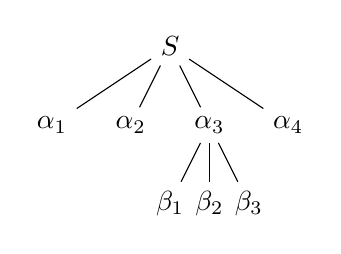
\begin{tikzpicture}
\node (S) at (0,5) {$S$};
\node (a1) at (-1.5,4) {$\alpha_1$};
\node (a2) at (-0.5,4) {$\alpha_2$};
\node (a3) at (0.5,4) {$\alpha_3$};
\node (a4) at (1.5,4) {$\alpha_4$};
\node (b1) at (0,3) {$\beta_1$};
\node (b2) at (0.5,3) {$\beta_2$};
\node (b3) at (1,3) {$\beta_3$};
\draw (S) edge (a1) edge (a2) edge (a3) edge (a4);
\draw (a3) edge (b1) edge (b2) edge (b3);
\end{tikzpicture}
\end{center}
We keep going until all leaves are labelled by terminals, then extend all the terminals straight down to the same level.

For instance, in the bracket language, for the word $(()(()))$ with productions $S \to (S)|SS|()$.
\begin{center}
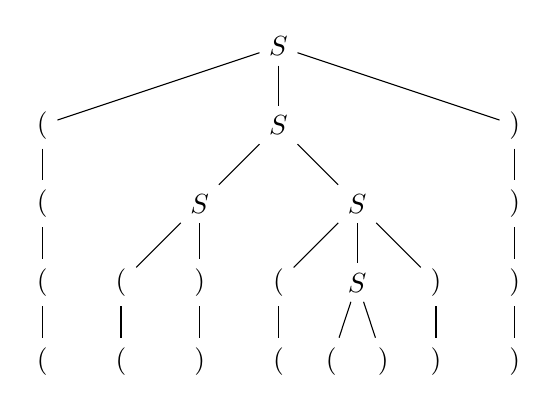
\begin{tikzpicture}
\node (S) at (0,5) {$S$};
\node (a1) at (-3,4) {$($};
\node (a2) at (-0,4) {$S$};
\node (a3) at (3,4) {$)$};
\node (b1) at (-3,3) {$($};
\node (b2) at (-1,3) {$S$};
\node (b3) at (1,3) {$S$};
\node (b4) at (3,3) {$)$};
\node (c1) at (-3,2) {$($};
\node (c2) at (-2,2) {$($};
\node (c3) at (-1,2) {$)$};
\node (c4) at (0,2) {$($};
\node (c5) at (1,2) {$S$};
\node (c6) at (2,2) {$)$};
\node (c7) at (3,2) {$)$};
\node (d1) at (-3,1) {$($};
\node (d2) at (-2,1) {$($};
\node (d3) at (-1,1) {$)$};
\node (d4) at (0,1) {$($};
\node (d5) at (0.67,1) {$($};
\node (d6) at (1.33,1) {$)$};
\node (d7) at (2,1) {$)$};
\node (d8) at (3,1) {$)$};

\draw (S) edge (a1) edge (a2) edge (a3);
\draw (a2) edge (b2) edge (b3) (a1) edge (b1) (a3) edge (b4);
\draw (b1) edge (c1) (b2) edge (c2) edge (c3) (b3) edge (c4) edge (c5) edge (c6) (b4) edge (c7);
\draw (c1) edge (d1) (c2) edge (d2) (c3) edge (d3) (c4) edge (d4) (c5) edge (d5) edge (d6) (c6) edge (d7) (c7) edge (d8);
\end{tikzpicture}
\end{center}

Note that if $G$ is a CFG in CNF then a parse tree as $\leq 2^i$ symbols on level $i$ as each vertex has at most $2$ descendents.

\begin{theorem}[Pumping Lemma for CFLs]
Let $L$ be a CFL. Then there is some $n$ such that for every word $u \in L$ with $|u| \geq n$, we can write $u$ as 5 subwords $u=vwxyz$ such that:
\begin{enumerate}
\item $w$ and $y$ are not both $\epsilon$
\item $|wxy|\leq n$
\item $\forall k \geq  0$ we have $vw^kxy^kz \in L$.
\end{enumerate}
\end{theorem}
\begin{proof}
We can take a CFG $G$ for $L$ in Chomsky normal form. Take $n=2^{m+1}$ for $m =|N|$, the number of nonterminals in $G$. 

If $u \in L$ and $|u| \geq n$ then any parse tree for $u$ has depth $\geq m+1$. Let $\Pi$ be a path from the root down to the last level passing only through nonterminal vertices except the finial vertex. Let $A$ be the first repeated nonterminal going from the bottom to the top. Note that this must happen since $m+1>m$. If we use the lower $A$ vertex as a root for the subtree below it, regarded as a smaller parse tree with start symbol $A$, we obtain some word $x \in \Sigma^{\ast}$. If we do the same with the upper $A$ we obtain $wxy \in \Sigma^{\ast}$. Note that $|wxy|>|x|$, so $w, y$ are not both $\epsilon$. Also the upper subtree has depth $\leq m+1$, and so $|wxy|\leq n$. Then we simply replace the lower $A$ by the upper $A$, and repeat $k$ times to get $vw^kxy^kz$. Alternatively, replace top $A$ by lower $A$ and pump down to $vxz$.
\end{proof}

\section{Nondeterministic Pushdown Automata}
NPDAs are to CFLs as NFAs are to regular languages. We read letters from the input word $w \in \Sigma^{\ast}$. We then have a staccyboi and doot doot around between some states. Our stackotron has as much memry as you want you greedy nerd, but can only hang on to symbols of some alphabet $\Gamma$ read LIFO because its a stacc and that's what a frickin stack does y'ken. Then when we wanna swerve around the states like a total madman we gots 3 pieces of info to use: the letter we is on, the state we is on, and the top of that stackawhack. Our transitionyboi $\delta$ can also tell us what we should be yeeting ourselves off to, what to yeet onto the top of that pile of juicy letters. In terms of notatatatation we draw our stack like a lil pole on top of a floor or something idk ig it's an upside down $T$, sorta like this hunny: $\bot$. We can make all $\epsilon$-NFAs into these chickydoodas by just ignoring the stacc like my crush ignores me.
\begin{theorem}
$L$ is a CFL $\iff$ it is the language of an NPDA
\end{theorem}
\begin{corollary}
A reglar language is context free
\end{corollary}
\begin{proof}
Lol nope we ain't provin any of this here
\end{proof}
\end{document}